\documentclass[11pt, aspectratio=169]{beamer}

% LuaLaTeXで日本語を使うための必須パッケージ
\usepackage{luatexja}

% 便利な追加パッケージ
\usepackage{booktabs}   % 表の罫線
\usepackage{tikz}       % 図形描画
% 以下の行を追加
\usetikzlibrary{shapes.symbols, shapes.geometric, arrows.meta, positioning}
\usepackage{listings}   % ソースコード挿入
\lstset{
  basicstyle=\ttfamily\scriptsize,
  frame=single,
  breaklines=true,
  numbers=left,
  numberstyle=\tiny
}

% テーマとカラーテーマの設定
\usetheme{Madrid}
\usecolortheme{orchid}

% ==========================================
% 【改良】セクション・サブセクションの可視化設定
% ==========================================

% 1. セクション開始時の自動表紙（大きな扉絵）
\AtBeginSection[]{
  \begin{frame}
    \vfill
    \centering
    \begin{beamercolorbox}[sep=8pt,center,shadow=true,rounded=true]{title}
      \usebeamerfont{title}\insertsectionhead\par%
    \end{beamercolorbox}
    \vfill
  \end{frame}
}

% 2. サブセクション開始時に「現在のセクション内の目次」を自動挿入
% 今いるサブセクション以外を半透明（shaded）にすることで、現在地が強調されます
\AtBeginSubsection[]{
  \begin{frame}{\insertsectionhead}
    \tableofcontents[currentsection, currentsubsection, subsectionstyle=show/shaded/hide]
  \end{frame}
}

% タイトル情報
\title{Webと管理}
\subtitle{HTTPの仕組みとその他}
\author{学籍番号(Student ID): 1280391 \\ 氏名(Name): 細川夏風(Hosokawa Natsuka)}
\institute{高知工科大学(Kochi Univ of Tech)}
\date{\today}

\begin{document}

\tikzstyle{client} = [rectangle, rounded corners, draw=blue!60, fill=blue!10, very thick, minimum width=2.5cm, minimum height=1.5cm, align=center]
\tikzstyle{server} = [rectangle, rounded corners, draw=green!60!black, fill=green!10, very thick, minimum width=2.5cm, minimum height=1.5cm, align=center]
\tikzstyle{internet} = [cloud, cloud puffs=12, cloud puff arc=120, aspect=2, draw=gray, fill=gray!10, very thick, minimum width=3.5cm, minimum height=2cm, align=center]
\tikzstyle{arrow} = [-{Stealth[scale=1.2]}, thick, draw=black!80]

% タイトルスライド
\begin{frame}
    \titlepage
\end{frame}

% 全体目次スライド
\begin{frame}{目次}
    \tableofcontents
\end{frame}

% ==========================================
% ここから本文
% ==========================================

\section{WWW(World Wide Web)}

\subsection{基本概念}
\begin{frame}{基本概念}
  \begin{columns}
    \begin{column}{0.48\textwidth}
      \texttt{WWW(World Wide Web)}はインターネット上の情報をハイパーテキスト形式で参照できるシステム．近年は単に\texttt{Web}と呼ばれることが多い．この情報を画面に表示するソフトウェアとして\texttt{Web}ブラウザが存在する．

      \texttt{Web}は大きく$3$つの定義がある．
      \begin{itemize}
        \item 情報へのアクセス手段と位置の定義: \texttt{URI(Uniform Resource Identifier)}
        \item 情報の表現フォーマットの定義: \texttt{HTML(Hyper Text Markup Language)}
        \item 情報の転送などの操作の定義: \texttt{HTTP(Hyper Text Tranceder Protocol)}
      \end{itemize}
    \end{column}
    \begin{column}{0.48\textwidth}
      \begin{tikzpicture}[node distance=0.6cm and 0.6cm]

        % ノードの配置（さらに小さく設定）
        \node [client, minimum width=1.8cm, minimum height=0.8cm, font=\scriptsize] (browser) {クライアント\\(Webブラウザ)};
        \node [internet, minimum width=2.4cm, minimum height=1.2cm, font=\scriptsize] (net) [below=of browser] {インターネット};
        \node [server, minimum width=1.8cm, minimum height=0.8cm, font=\scriptsize] (webserver) [below=of net] {Webサーバ};

        % HTTPリクエスト（右側を曲線で通る）
        % [bend left=40] で少し強めに曲げて矢印の膨らみを抑えます
        \draw [arrow] (browser.east) to[bend left=40] node[right, font=\tiny] {HTTPリクエスト} (net.east);
        \draw [arrow] (net.east) to[bend left=40] node[right, font=\tiny] {HTTPリクエスト} (webserver.east);

        % HTTPレスポンス（左側を曲線で通る）
        \draw [arrow] (webserver.west) to[bend left=40] node[left, font=\tiny] {HTTPレスポンス} (net.west);
        \draw [arrow] (net.west) to[bend left=40] node[left, font=\tiny, align=center] {HTTPレスポンス\\(HTML, 画像等)} (browser.west);

      \end{tikzpicture}
    \end{column}
  \end{columns}
\end{frame}

\subsection{URI}
\begin{frame}{URIについて}
  \texttt{URI}は資源を表す表記法(識別子)として利用され，\texttt{WWW}以外にも用いることのできる汎用性の高い識別子である．

  下記の例に示した\texttt{URL(Uniform Resouce Locator)}も存在し，これは俗に「ホームページのアドレス」を指す．

  \begin{exampleblock}{\texttt{URL}の例}
    \begin{itemize}
      \item \texttt{https://www.google.com              \#GoogleのURL}
      \item \texttt{https://www.kochi-tech.ac.jp/       \#KUTのURL}
    \end{itemize}
  \end{exampleblock}
  \texttt{URI}の\texttt{http}スキームの書式は次にようになっている．
  \begin{block}{\texttt{http}スキームの構成}
    \begin{itemize}
      \item \texttt{http://}ホスト名\texttt{:}ポート番号\texttt{/}パス\texttt{?}問い合わせ内容\texttt{\#}部分情報
    \end{itemize}
  \end{block}
\end{frame}

\begin{frame}{主なURIスキーム}
  \begin{table}
    \centering
    \caption{主な URI スキーム（抜粋）}
    \begin{tabular}{ll}
      \hline
      \textbf{スキーム名} & \textbf{内容} \\
      \hline
      file & Host-specific File Names \\
      ftp & File Transfer Protocol \\
      http & Hypertext Transfer Protocol \\
      https & Hypertext Transfer Protocol Security \\
      mailto & Electronic Mail Address \\
      tel & Telephone \\
      urn & Uniform Resource Name \\
      \hline
    \end{tabular}
  \end{table}
\end{frame}

\subsection{HTML}
\begin{frame}[fragile]{HTML}
  \begin{columns}
    \begin{column}{0.44\textwidth}
      \texttt{HTML}は\texttt{Web}ページを記述するための言語(データ形式)である．ブラウザの画面に文字や位置，音や画像，動画の設定ができる．また，\texttt{HTML}にはハイパーテキストと呼ばれる機能があり，画面に表示される文字や絵にリンク(link)と呼ばれる情報を貼り付けられる．これにをクリックすると別の情報を表示したり，別のページに移行することができる．
    \end{column}
    \begin{column}{0.48\textwidth}
      \begin{lstlisting}[basicstyle=\ttfamily\tiny, title={HTMLの記述例}]
<!DOCTYPE HTML PUBLIC "-//W3C//DTD HTML 4.01 Transitional//EN"
  "http://www.w3.org/TR/html4/loose.dtd">
<html lang="ja">
<head>
  <meta http-eqiv="Content-Type" content="text/html; charset=UTF-8">
  <title>Mastaring TCP/IP</title>
</head>
<body>
<h1>「マスタリングTCP/IP」紹介ページ</h1>
<img src="cover.jpg" alt="マスタリングTCP/IPカバーイメージ">
<ul>
  <li><a href="feature.html">マスタリングTCP/IPの特徴</a></li>

</ul>
</body>
</html>
      \end{lstlisting}
    \end{column}
  \end{columns}
\end{frame}

\subsection{HTTP}
\begin{frame}{HTTP}
  ユーザが\texttt{Web}ページの\texttt{URI}を入力すると\texttt{HTTP}の処理が開始され専用のポートが利用され，通信が確立される．その通信路を利用してコマンドや応答，データからなるメッセージの送受信が行わる．

  \begin{block}{HTTPのコマンドと応答メッセージの意味}
    コマンド(サイト上ではリクエストメソッド)
    \begin{itemize}
      \item \texttt{https://qiita.com/morikuma709/items/956d7c58908cb481d7e8}
    \end{itemize}
    応答メッセージ番号の意味
    \begin{itemize}
      \item \texttt{https://qiita.com/takuo\_maeda/items/9cff0b03e74f8f600eee}
    \end{itemize}
  \end{block}
\end{frame}

\begin{frame}{HTTPのバージョンによる違い}
  \begin{itemize}
    \item \texttt{HTTP/1.0}
      \begin{itemize}
        \item ヘッダーが導入され，テキスト以外の送受信が可能に
      \end{itemize}
    \item \texttt{HTTP/1.1}
      \begin{itemize}
        \item 1度の\texttt{TCP}接続を維持し，複数のリクエストとレスポンスで使い回せるようになった．
      \end{itemize}
    \item \texttt{HTTP/2}
      \begin{itemize}
        \item 1つの通信の中で順番待ち無く並行的に通信を行うことができるようになった．
      \end{itemize}
    \item \texttt{HTTP/3}
      \begin{itemize}
        \item \texttt{TCP}では無く，\texttt{UDP}で\texttt{HTTP}通信を行うという方式を採用することによって通信の高速化を実現．
      \end{itemize}
  \end{itemize}
\end{frame}

\subsection{Javascript，CGI，Cookie}
\begin{frame}{現代のWebに用いられる技術}
  \begin{itemize}
    \item \textbf{\texttt{Javascript}}

      \texttt{Javascript}は\texttt{HTML}に埋め込めるプログラミング言語で\texttt{Web}ブラウザ上で動作する．\texttt{Javascript}が埋め込まれた\texttt{HTML}をダウンロードするとプログラムがクライアント側で実行される．これにより，テキストボックスの未入力の検知などに使われる．更には近年は\texttt{Javascript}で\texttt{DOM}を操作し，動的なサイトを作ることも可能となっている．
      
    \item \textbf{\texttt{CGI}}

      \texttt{CGI}は，サーバが外部のプログラムを呼び出し，その結果を\texttt{HTML}上に反映することによって，静的なものに限定されず動的なサイトを制作することができる．

    \item \textbf{\texttt{Cookie}}

      \texttt{Web}アプリケーションでは，ユーザ情報の識別のため，この仕組みが用いられる．\texttt{Cookie}は\texttt{Web}サーバがクライアント情報(タグ名とタグ名につける値)を格納するために使用される．買い物情報などの様々な情報をブラウザに記憶させることができる．
  \end{itemize}
\end{frame}

\section{その他}

\subsection{SNMP}
\begin{frame}{SNMP(Simple Network Management Protocol)}
  \texttt{SNMP}は\texttt{UDP/IP}上で動作するプロトコルでネットワーク管理に用いられる．
  管理する側をマネージャ(\texttt{NW}監視端末)，管理される側をエージェント(ルータやスイッチのこと)と呼ぶ．
  マネージャががエージェントに対して
  \begin{itemize}
    \item 情報の参照要求
    \item 情報の設定要求
  \end{itemize}
  エージェントがマネージャに対して
  \begin{itemize}
    \item 要求に対する返答
    \item イベンの通知
  \end{itemize}
  を行うことによってネットワークの管理を最適化する．

  このときやり取りされる情報に\texttt{MIB(Management Information Base)}があり，これはツリー構造のデータベースであり，番号が割り振られている．マネージャはこの値を更新したり，取り出したりすることによってエージェントの情報を読み取ったり操作することができる．
\end{frame}

\subsection{その他のアプリケーションプロトコル}
\begin{frame}{マルチメディアのプロトコル}
  \begin{itemize}
    \item H.322

      \texttt{ITU}によって標準化された．\texttt{TCP/IP}ネットワーク上でリアルタイムに音声，動画を交換するためのプロトコル．通話システム全体の仕様を定めたもの．

    \item \texttt{SIP(Session Initation Protocol)}

      マルチメディア通信を行うためのプロトコル．複数人でのセッションの作成等を行うことができる．セッション層に相当すると考えられる．

    \item \texttt{RTP(Real-time Transport Protocol)}

      音声やビデオなどリアルタイムデータを\texttt{UDP}を用いて通信を行う際，的確に通信を行うためのプロトコル．
  \end{itemize}
\end{frame}

\begin{frame}{P2P(Peer To Peer)}
  \begin{columns}
    \begin{column}{0.48\textwidth}
      現代のインターネットの通信の殆どは1対$N$のクライアント・サーバシステムがほとんどである．

      しかし，そうでない方法として\texttt{P2P}という方法が存在する．これは端末がホストやサーバを介さず，1対1で直接通信を行う仕組みである．各端末がクライアントとサーバの両方の機能を持つ対等なサービスである．
      
      この仕組みにもデメリットが存在する．それが互いの端末がインターネットからアクセス可能な場所になければならないことである．現代においてはローカル\texttt{IP}などの仕組みが存在するため，\texttt{NAT}を超えて通信を行える仕組みが必要である．
    \end{column}
    \begin{column}{0.48\textwidth}
      \begin{figure}
        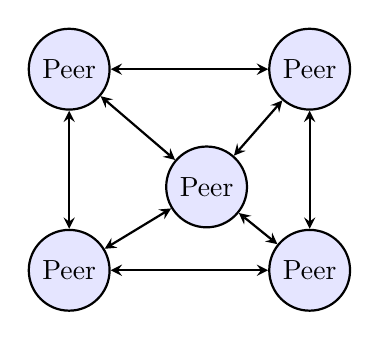
\begin{tikzpicture}[
          peer/.style={draw, circle, minimum size=1.0cm, align=center, thick, fill=blue!10},
          >=stealth,
          thick
        ]
          % ノードの配置
          \node[peer] (p1) {Peer};
          \node[peer] (p2) [right=2cm of p1] {Peer};
          \node[peer] (p3) [below=1.5cm of p1] {Peer};
          \node[peer] (p4) [below=1.5cm of p2] {Peer};
          \node[peer] (p5) [below right=0.75cm and 1cm of p1] {Peer};

          % 双方向の通信（エッジ）
          \draw[<->] (p1) -- (p2);
          \draw[<->] (p1) -- (p3);
          \draw[<->] (p1) -- (p5);
          \draw[<->] (p2) -- (p4);
          \draw[<->] (p2) -- (p5);
          \draw[<->] (p3) -- (p4);
          \draw[<->] (p3) -- (p5);
          \draw[<->] (p4) -- (p5);
        \end{tikzpicture}
        \caption{中央サーバーを持たず端末同士が対等に通信するモデル}
      \end{figure}
    \end{column}
  \end{columns}
\end{frame}

\end{document}
